\documentclass[journal]{IEEEtran}
\usepackage[a5paper, margin=10mm, onecolumn]{geometry}
\usepackage{amsmath,amssymb,amsfonts}
\usepackage{graphicx}
\usepackage{enumitem}
\usepackage{hyperref}
\begin{document}

\title{11.16.3.6}
\author{EE24BTECH11004 - Ankit Jainar}
\maketitle

\textbf{Question:}
There are four men and six women on the city council. If one council member is selected for a committee at random, how likely is it that it is a woman?

\section*{Theoretical Solution}
The total number of council members is:
\begin{align}
    |S| = 4 + 6 = 10
\end{align}
The favorable outcomes (selecting a woman) are:
\begin{align}
    |A| = 6
\end{align}
The probability of selecting a woman is:
\begin{align}
    P(A) = \frac{|A|}{|S|} = \frac{6}{10} = 0.6
\end{align}

\section*{Introduction}
This task involves simulating the random selection of council members using a C program, compiling it into a shared object (.so) file, and using Python to process the results and generate a probability distribution plot.

\section*{C Code Description}
The C program generates random samples for the selection process, where the outcomes are categorized as either man or woman. The program uses the \texttt{rand()} function to simulate the random selection and increments a counter for each outcome.

\section*{Python Code Description}
The Python code performs the following:
\begin{enumerate}
    \item Loads the shared object file generated from the C program using the \texttt{ctypes} library.
    \item Simulates a specified number of random selections (e.g., 1,000,000 trials).
    \item Calculates the probability of selecting a woman using the formula:
    \begin{align}
    P(\text{woman}) = \frac{\text{frequency of selecting a woman}}{\text{total trials}}
    \end{align}
    \item Plots the probability distribution using \texttt{matplotlib}.
\end{enumerate}

\section*{Graphical Output}
The Python code generates a bar chart where:
\begin{itemize}
    \item The x-axis represents the outcomes: Man and Woman.
    \item The y-axis represents the probabilities, ranging from 0 to 1.
    \item The bar height for Woman corresponds to the probability $P(A) = 0.6$.
\end{itemize}

\section*{Stemplot Distribution}
The stemplot shows a single vertical line at Woman on the x-axis with a height corresponding to its probability (0.6).
\subsubsection*{Probability Mass Function (PMF)}
The PMF represents the probability of each individual outcome in the sample space \( S \). For the city council:
\[
S = \{\text{Man, Woman}\},
\]
the PMF is given as:
\[
P(X = x) = 
\begin{cases} 
\frac{6}{10}, & x = \text{Woman}, \\ 
\frac{4}{10}, & x = \text{Man}, \\ 
0, & x \notin S.
\end{cases}
\]

\subsubsection*{Cumulative Distribution Function (CDF)}
The CDF represents the cumulative probability of outcomes up to a given value \( x \), defined as:
\[
F(x) = P(X \leq x) = \sum_{k \in S, k \leq x} P(X = k).
\]
For the city council:
\[
F(x) = 
\begin{cases} 
0, & x < \text{Man}, \\ 
\frac{4}{10}, & x = \text{Man}, \\ 
1, & x \geq \text{Woman}.
\end{cases}
\]

\subsection*{Simulation Process}
We simulate the selection of a council member using the following steps:
\begin{enumerate}
    \item The city council consists of members in the set:
    \[
    S = \{\text{Man, Woman}\},
    \]
    with 4 men and 6 women.
    \item For each simulated selection, a random integer \( X \) is generated such that:
    \[
    X \in \{1, 2, 3, \dots, 10\},
    \]
    using a random number generator function:
    \[
    X = (\text{rand()} \mod 10) + 1.
    \]
    \item If \( X \leq 6 \), it corresponds to a woman; otherwise, it corresponds to a man.
    \item The number of occurrences of each outcome is tracked over \( N \) trials, where \( N \) is the total number of simulations.
    \item Both the PMF and CDF are computed:
    \begin{itemize}
        \item **PMF**: The frequency of selecting a woman or a man is divided by the total number of trials to compute the probabilities.
        \item **CDF**: The cumulative probabilities are calculated as the running total of the PMF values.
    \end{itemize}
\end{enumerate}

\subsection*{Calculation of Probabilities}
\subsubsection*{Probability of Selecting a Woman (PMF)}
The probability of selecting a woman is computed as:
\[
P(\text{Woman}) = \frac{\text{Number of women}}{\text{Total council members}} = \frac{6}{10} = 0.6.
\]

\subsubsection*{Cumulative Probability (CDF)}
The cumulative probability of selecting up to a given member type is:
\[
F(x) = 
\begin{cases} 
P(\text{Man}), & x = \text{Man}, \\ 
P(\text{Man}) + P(\text{Woman}), & x = \text{Woman}.
\end{cases}
\]
For the city council:
\[
F(\text{Man}) = 0.4, \quad F(\text{Woman}) = 1.
\]

\subsubsection*{Probability of Selecting \( X \notin S \)}
Since all members of the council belong to the set \( S = \{\text{Man, Woman}\} \), the probability of selecting \( X \notin S \) is:
\[
P(X \notin S) = 0.
\]

\subsection*{Output Representation}
The computed probabilities are represented in two forms:
\begin{itemize}
    \item PMF: The probabilities of selecting each type of council member (\text{Man, Woman}).
    \item CDF: The cumulative probabilities up to each member type (\text{Man, Woman}).
\end{itemize}


\section*{Conclusion}
This task demonstrates the integration of C and Python for simulating and visualizing a probabilistic experiment. The probability of selecting a woman from the council is calculated as \textbf{0.6}, matching the theoretical value.


\begin{figure}[h!]
   \centering
   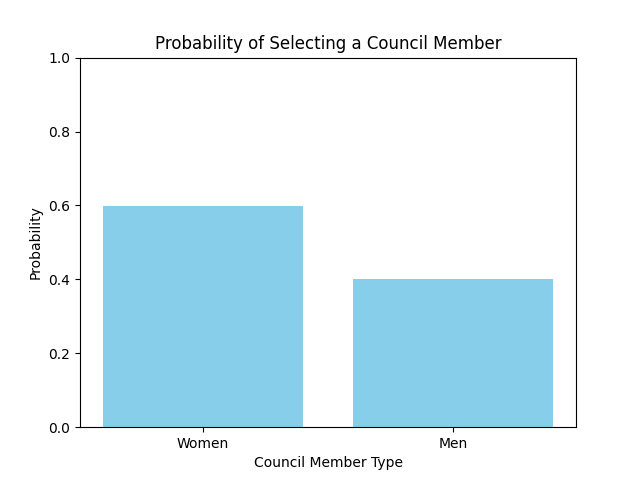
\includegraphics[width=\columnwidth]{figs/fig1.png}
   \end{figure}
\begin{figure}[h!]
   \centering
   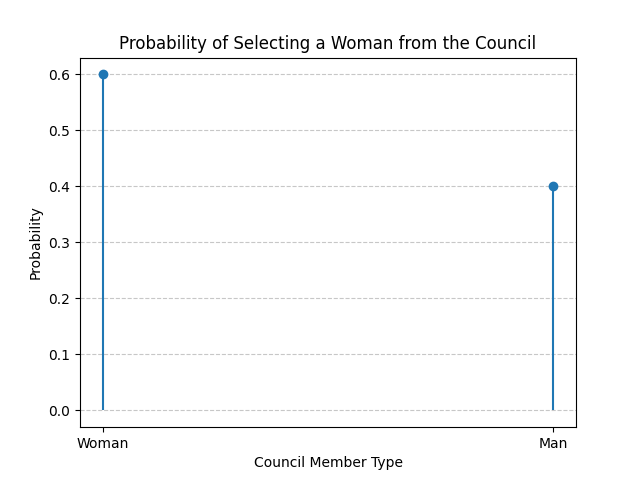
\includegraphics[width=\columnwidth]{figs/fig2.png}
   \end{figure}
\begin{figure}[h!]
   \centering
   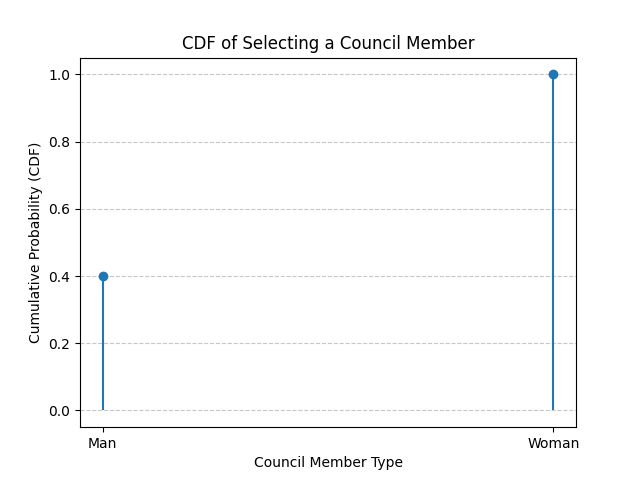
\includegraphics[width=\columnwidth]{figs/fig3.png}
   \end{figure}

\end{document}

